\chapter{Introduction, State-of-the-art and proposed contributions}
\label{chap:Litreview}
% preferred location for \figurepath in this chapter
\setfigurepath{figures/Litreview}
The present thesis is partially supported by the RTE company through the RTE/UPMC Chair of ``\textit{Intervention Robotics}" held by Vincent Padois. The intended goal of this chair is to bring new insights for the development of intervention robotic systems and assistant robots capable of safely interacting with humans. Within this context, the work presented hereby focuses especially on the control problem.
\section{Motivation}
Despite their matured technology, robotic solutions are still underused in many industrial contexts. These contexts include for example the aeronautics and shipbuilding industries, the construction and energy production domains, and the small and medium-sized enterprises (SMBs) operating in a flexible craft mode rather than in a standardized manufacturing mode. Several reasons, when combined, can explain the low presence of robots in these areas: 
\begin{enumerate}
\item the complex nature of the tasks to be performed, which require a technical and gestural expertise of one or several human-operators;
\item the complexity and dynamics of partially or fully unstructured environments in which it is difficult, if not impossible, to place a robot and still be able to guarantee safety for nearby humans;
\item the cost of dedicated robotic solutions.
\end{enumerate}
An efficient way of introducing robots in these domains is to consider the use of robots as \textit{collaborative} tools which tasks are defined \textit{on the fly} and can be adapted online through simple interaction with humans. For example, it is possible to combine the gestural expertise of an operator and his skills for solving problems and taking decisions with the payload, precision and repeatability performances of a robot. This so-called ``\textit{collaborative}" robotics is a subject of growing attention in the fields of industrial and academic robotics. Nevertheless, it poses fundamental questions that remain so far open:
\begin{enumerate}[label=\Alph*)]
\item how to guarantee on-line the existence of a solution to the control problem when the task is not defined a priori by planning or when it is adapted in real-time as a reaction to a dynamic environment? Indeed, in conventional applications of robotics, tasks are defined a priori and off-line planning can ensure that all the mechanical and actuation related constraints inherent to the physical capabilities of the robot are not violated by the achieved movements. This is no longer the case when the task is not defined off-line and it becomes necessary to ensure that the retained command decision at each time-step in order to perform the task in the most optimal way will not ultimately lead to inevitable constraints violation.
\item How to ensure the safety of the environment in cases where: i) Geometric collision avoidance cannot be guaranteed (the robot has a fixed base and cannot escape to avoid collisions). ii) Unanticipated physical interaction is an acceptable scenario for short periods of time (e.g., when a human intersects with the trajectory of a robot in motion)? This topic is referred to in the literature as ``Physical Human-Robot Interaction (pHRI)" and it is the first branch of the broader topic of ``\textit{Human-Robot Interaction}" \cite{albu2005physical}.
\item Beyond the implementation of robust interactive control laws and the problem of safety that must be handled during physical interaction, how is it possible to simplify/facilitate cognitively the sharing of tasks between a robot and a human? Indeed, providing robots with the capability of predicting humans behaviour by estimating their affective state can considerably improve the quality of human-robot interaction. Acquired data like verbal and non verbal signals for example facial expressions and the ``body language" can be used to adapt the robot actions and make its interaction with humans more effective and intuitive \cite{kulic2007affective}, \cite{mavridis2015review}. This field that studies the ``social and Cognitive aspects of Human-Robot Interactions (cHRI)" is the second branch of the ``\textit{Human-Robot interaction}" topic.
\end{enumerate}
The present thesis provides new insights regarding the problems described in A) and B). First, it addresses a problem referred to in the literature as \textit{constraints incompatibility}. This problem occurs for reactive controllers, i.e., control problems where the task to perform is not known in advance but discovered in real-time, when the formulation of the constraints (e.g., constraints related to the physical limitations of a robot actuators) the robot must cope with does not take into account the dynamic capabilities of its actuators. The solvability of the control problem in such cases cannot be ensured for the present and future states of the robot. The problem of \textit{constraints incompatibility} in the joint space is solved in the first part of the work presented in this thesis. The second part focuses on the peculiar aspects of ``physical" human-robot interaction with safety as a main criteria for developing a new control strategy. The proposed controller uses the amount of energy deployed by the robot to asses and limit its degree of danger towards a nearby human-operator during different interaction phases: at the establishment/during physical contact, in case of non-deliberate collisions and when physical contact is released. \\
The rest of this chapter is organized as follows: first, state-of-the-art mechanical designs, control strategies and safety standards used to handle safety during human-robot interaction are briefly outlined and used to position the presented work. Then, the problems tackled in each chapter are furthermore detailed and finally, the different contributions are summarized.
%%%%%%%%%%%%%%%%%%%%%%%%%%%%%%%%%%%%%%%%%%%%%%%%%µµµµµµµµµµ
\section[Safe mechanical design]{Safety oriented mechanical design}
Traditionally in robots, stiff actuators governed by the principle of ``the stiffer, the better'' are used for tasks requiring tracking of a desired trajectory with high accuracy \cite{salisbury1991design}. When these are perfect for such use, they pose however various fundamental problems for applications requiring interaction with unknown and dynamic environments including humans. These robots cannot just blindly move along computed trajectories without concern of the induced forces caused by contacts with the environment. They must be able to properly and safely react to such perturbations. Challenges related to the interaction of a robot with its environment can partially be tackled from a control point of view, but to reach human like compliance capabilities without sacrificing much of the machines performances, the entire robotic design must be reconsidered. Indeed, researchers have quickly realized that in humans not only the brain creates the intelligence of the body, but also the morphology and biomechanics of the muscles play a critical role in the way humans think and move \cite{pfeifer2006body}. Therefore, besides the proprioceptive sensors, such as Cartesian force/torque sensors, articular torque sensors and tactile sensitive skins \cite{Fogale-url}, back-drivable motors can be used to passively react to external forces \cite{townsend1993mechanical} and subsequently, intrinsically flexible actuators inspired from the biological spring-like properties of human muscles became a subject of interest \cite{burdet2001central}.  
%%%%%%%%%%%%%%%%%%%%%%%%%%%%%%%%%%%%%%%%
\subsection{Flexible actuators}
Despite the tradition of making the interface between an actuator and its load as stiff as possible, reducing this stiffness has a number of advantages that can bring the actuation closer to human capabilities. This can result into: greater shock tolerance, lower reflected inertia by decoupling the motor side from the link-side inertia, more stable and accurate force control in addition to the capacity for storing and releasing energy \cite{garabini2011optimality}, \cite{chen2013optimal}. Depending on how their stiffness and damping are achieved, intrinsically flexible actuators can be divided into two main categories \cite{vanderborght2012variable}: \\
\begin{itemize}
\item Actuators with emulated compliance, where the impedance (stiffness and/or damping) of the actuator can be adjusted using software control and joint level torque sensing \cite{loughlin2007dlr}. The main advantage of such actuators is the possibility to tune the desired elasticity parameters online so the mechanical behaviour can be adapted for different tasks. On the other hand, as no physical compliant element is present, energy cannot passively be stored in the system. Active compliance has been pioneered by the DLR and is today commercialized in Kuka robotic systems \cite{bischoff2010kuka}. This technology has also been shown in hydraulic actuators on systems such as Sarcos \cite{hyon2007full} and the hydraulically actuated quadruped robot HyQ \cite{boaventura2012dynamic}.
\item Actuators with inherent compliance that contains a passive flexible element where the effective joint impedance is altered via active control. Such designs started with earlier VIA (Variable Impedance Actuators) such as Mckibben pneumatic actuators \cite{caldwell1995control} and the famous series elastic actuator (SEA) \cite{pratt1995series}, \cite{laffranchi2011compact}, \cite{vanderborght2013variable} (see Fig.~\ref{fig:SEA}). This category can be divided into two main design approaches: i) Mechanisms where the mechanical compliance of the element cannot be changed (fixed compliance). For example the Tsagarakis et al. \cite{tsagarakis2009compact} ComPact soft actuator for the iCub robot that uses 6 linear springs and the HypoSEA \cite{ivar2011nonlinear} designed to stretch a linear spring in a non-linear way. ii) Adaptable compliance systems where the stiffness is controlled by mechanical reconfiguration. In this case, usually two motors are used: one to control the equilibrium position of the joint and a second to control its compliance. A famous example of such design is the DLR
Floating Spring Joint (FSJ) \cite{wolf2011dlr} designed for the first 4 axes of the anthropomorphic DLR Hand Arm System \cite{grebenstein2011dlr}. \\
To help tuning passive elasticity for actuators, Kashiri et al in \cite{kashiri2013stiffness} introduced a method for the selection of passive stiffness of compliant actuated arms. The method is based on the effects of passive compliance on key parameters including natural frequency, damping ratio, Cartesian stiffness and energy storage capacity.
\end{itemize}
More details about VIAs and their various design technologies can be found in \cite{vanderborght2013variable} and among the VIACTORS project \cite{VIACTORS-url} related publications. 
\begin{figure}[!ht]
\centering

\includegraphics[width=0.65\linewidth]{\figurepath/SEA}
\caption{Bloc diagram of Series Elastic actuators.}
\label{fig:SEA}
\end{figure} 
%%%%%%%%%%%%%%%%%%%%%%%%%%%%%%%%%%%%%%%%%%%%%%%%%
\subsection{Lightweight Robotic Systems}  
Using the aforementioned actuation technology, robots based on lightweight and highly integrated mechatronics designs that are more suitable for physical interaction with humans have been developed. Prominent state-of-the-art robots from this category are depicted in Fig.~\ref{fig:robots}: 
\begin{figure}[!ht]
\centering
\includegraphics[width=1\linewidth]{\figurepath/robots}
\caption{(a) KUKA LBR iiwa, (b) Franka Emika arm, (c) Universal Robots UR10, (d) ABB YuMi and (e) Rethink Robotics Sawyer.}
\label{fig:robots}
\end{figure} 
%The Barrett arm
%The Mitsubishi PA10
The KUKA LBR iiwa \cite{iiwa-url} is a fully torque controlled robot designed as a continuation of the DLR lightweight robotic arms lineup. Based on the DLR LWR-III, it has 7 degrees of freedom, weighs $14~kg$ and is able to achieve a unitary payload-to-weight ratio. In addition to its torque sensors at each joint, the robot is equipped with redundant joint position sensors on both actuation and link sides. \\
%
Franka Emika \cite{Franka-url} is a highly cost competitive robotic arm also aimed for human-robot collaboration. Launched in 2017, despite its low cost, it has similar features to other more expensive systems. The robot is equipped with torque sensors in all its 7 joints and can handle payloads up to $3~kg$. \\
%
UR10 from UNIVERSAL ROBOTS \cite{UR10-url} is a commercially available lightweight redundant arm with a payload of $10~kg$. With only 6 degrees of freedom, it has however a great working range with joints that can perform  complete $+/-360~°$ rotations. \\
%
ABB Yumi is a collaborative dual-arm robot with 14 axes of freedom (7 in each arm) \cite{YuMi-url}. It includes flexible hands, parts feeding systems and embedded cameras. With a payload of $0.5~kg$, this robot is specifically designed for small parts assembly. \\
%
Sawyer is the latest robot model from Rethink Robotics. Based on the two armed Baxter, with 7 degrees of freedom, it exhibits better accuracy and repeatability performances \cite{Sawyer-url}. With embedded vision, the robot is able to handle loads up to $4~kg$ and thanks to its torque sensors, it can also be fully torque controlled. 

While other robot providers have recently started to propose collaborative versions of their standard robots, the five examples cited hereby remain forerunners of this domain.
%The system has a LED tablet as a face that can be used to render its interaction with humans more effective and intuitive.
%
%This is the case of robot manipulators actuated
%through pulleys and steel cables, where the elasticity is deter-
%mined by the elastic coefficient of the cables. Cable actuation can
%ensure human-like dimensions of the artifact, lightness and also
%anthropomorphic mass distributio
%%%%%%%%%%%%%%%%%%%%%%%%%%%%%%%%%%%%%%%%%%%%%%%%%
\section{Control}
%1)Parler des difrrentes techniques utuliser pour les controleurs d'interaction : ex force/position. 
%2)Parler du plus importaht qui est le impedance controller.
%3)Dire que sa formulation standart est por les robots stiff. 
%4)ensuite dire les problems que ça pose pour les robots élastiques. 
%5)Dires les nouvelles formulations.
%6) Parler des autres stratégie comme celle de sami. 
%
%
%The idea of extending human-like impedance control to robots aimed for physical interaction stared with the pioneering work of Hogan \cite{part1985impedance} The basic objective of such controllers is the achievement of a desired dynamical relation between external forces applied to the robot and its resulting movement. In many robotic  applications this dynamical behaviour is usually specified in terms  of stiffness and damping matrices with respect to some Cartesian  coordinates
%
%Which has since been extended to intrinsically flexible joint robots in [79, 16, 309, 15, 2015]
%
%
%A Passivity  Based Cartesian  Impedance  Controller for Flexible Joint Robots 
%- Part I: 
%/However in many robotic  applications this dynamical behaviour is specified in terms  of stiffness and damping matrices with respect to some Cartesian  coordinates 
%/A straight forward application of these techniques to a flexible joint robot  therefore usually will not  lead to a satisfactory performance'. In this paper an  impedance  control law is proposed  which 
%is designed for flexible joint robots. The desired  impedance is assumed to be  a  second  order  mass- spring-damper  system.  Furthermore only  the achievement of stiffness and  damping is  considered herein,  while  the inertial behaviour is left unchanged. 
%/However it has been shown that in practice only quite unsatisfactory results can be achieved with a restriction to purely motor position  (and velocity) based feedback controllers (without additional  non collocated  feedback) for the case of a  flexible joint robot. In some  works a controller structure based on a feedback of the joint torques as well as the link side positions was  considered and it  was  shown that this can lead to better results (see e.g. [IO]). This has  also  already been  verified experimentally with  the  DLR-light-weight-robots [2]
%
%
%
%A tank-based approach to impedance control with variable stiffness.
%The impedance control provides a compliant behaviour during the interaction and regulates the dynamic response of the robot end-effector to interaction forces by establishing a suitable virtual mass-spring-damper system on the end-effector
%Excessive contact force between the manipulator and the
%environment should be prevented. Since humans control the force exerted on an object by adapting their arm stiffness, in a similar way the robot should be able to change the stiffness of its arm while performing an interaction task. The
%/In order to imitate the surgeon’s behaviour, an impedance control with variable target stiffness is proposed in this paper
%/The contribution of this paper is a modified impedance
%control strategy that allows to reproduce a variable stiffness while preserving the passivity, and therefore a stable behaviour both in free motion and in interaction with partially known environments, of the robot.
%//Analogously to the stiffness of a human arm that is adapted for different tasks; [] propose a control strategy that allows to reproduce a variable stiffness while preserving the passivity and therefore a stable behaviour of the robot, both in free motion and during physical interaction.
%
%
%An  ISO10218-compliant  adaptive  damping  controller
%for  safe  Physical  Human-Robot  Interaction:
%the  International  Organization  for
%Standardization  included  requirements  for  a  safe  industrial
%robot.  This  standard  specifies  that  any  robot  must  respect
%velocity,  power  and  contact  force  limits  at  the  tool  control
%point (TCP) in the presence of a human
%//An  alternative  comes  from  control,  typically  impedance
%control [10], and its modified versions for force tracking [11],
%force  limitation  [12],  adaptive  damping  [13]  or  exploiting
%redundancy  [14].  However,  to  the  best  of  our  knowledge,
%the only work that explicitly tackles the ISO1028-2011 from a control viewpoint is [15].
%//In  this  paper,  we  propose  an  adaptive damping  controller  that  fulfills  the  ISO10218  requirements  by limiting  the  tool  velocity,  power  and  contact  force  online  (and only  when  needed
%//
%Adaptive Human–Robot Interaction Control for
%Robots Driven by Series Elastic Actuators:
%For the
%robot driven by SEAs, which closely interacts with humans, the
%interaction force between the human and the robot should be
%considered as an important safety measure, and it is necessary
%to control not only the position but also the interaction force. To
%realize the interaction control task, hybrid position/force con-
%trol [19] and impedance/admittance control [20]–[25] have been
%proposed for different robots.\\
For robots that physically interact with humans, the interaction force should imperatively be considered as an important safety quantifier \cite{ISO15066PDF}. It is thus necessary to control not only the position but also the interaction force \cite{ikuta2001safety}. To design an interaction oriented controller, the idea of force control has been an active research topic with initial work in \cite{whitney1977force} and \cite{mason1981compliance}. It can be divided into two main approaches \cite[Chapter~9]{siciliano2016springer}: 
\begin{itemize}
\item direct force control that uses an explicit closure of a force feedback loop. A widely adopted strategy from this category is hybrid force/position control that allows the user to simultaneously specify a desired motion along the unconstrained task directions and a desired contact force/moment along the constrained task directions \cite{raibert1981hybrid}, \cite{khatib1987unified}. A major concern with this approach is that for good performances, an accurate model of the contact properties of the environment of the robot is needed.
\item Indirect force control without explicit closure of a force feedback loop. Force control in this case is achieved via motion control. The most widely used scheme from this category is probably impedance control. The idea of extending human-like impedance control to robots aimed for physical interaction stared with the pioneering work of Hogan \cite{hogan1984impedance}. The basic objective of such controllers is the achievement of a desired dynamical relation between external forces applied to the robot and its resulting movement. In many robotic  applications this dynamical behaviour is specified in terms  of equivalent mass, stiffness and damping matrices with respect to some Cartesian coordinates \cite{ott2010unified}:
%\begin{equation}
%F_{ext} = M^*(\ddot{x}-\ddot{x}^*)+D^*(\dot{x}-\dot{x}^*)+K^*(x-x^*),
%\label{eq:impedance_cntrl}
%\end{equation}
%where $x$, $x^*$ $\in \mathbb{R}^{6}$ are the current and desired pose for the robot's end-effector, $F_{ext} \in \mathbb{R}^{6}$ is the external wrench (see Fig.~\ref{fig:damping_cntrl}) and $M^*, K^*, D^* \in \mathbb{R}^{6X6}$ are the desired Cartesian inertia, stiffness and damping matrices. 
\begin{equation}
F_{ext} = M^* \vect{\ddot{e}}+D^*\vect{\dot{e}}+K^*\vect{e},
\label{eq:impedance_cntrl}
\end{equation}
The terms $\vect{e}$, $\vect{\dot{e}}$ and $\vect{\ddot{e}}$ are not explicitly defined here because they are representation dependent (see \cite{Siciliano2008}). They respectively correspond to the position and orientation errors of the end-effector of the robot with respect to a desired pose $x^*$ and their first and second derivatives. $F_{ext} \in \mathbb{R}^{6}$ is the external wrench (see Fig.~\ref{fig:damping_cntrl}). $M^*, K^*, D^* \in \mathbb{R}^{6X6}$ are the desired Cartesian inertia, stiffness and damping matrices. 
\vspace*{-5mm}
\begin{figure}[H]
\captionsetup{width=.86\linewidth}
\centering
\includegraphics[width=0.35\linewidth]{\figurepath/damping_cntrl}
\caption{Desired mechanical behaviour expressed by a mass-spring-damper like system.}
\label{fig:damping_cntrl}
\end{figure} \\
\vspace*{-2mm}
Impedance control laws  provide accurate trajectory tracking in free motion while displaying passive properties (mass-spring-damper like system) in response to unexpected collisions. To overcome position tracking accuracy and stability problems when implementing impedance control for flexible joint robots, adapted schemes that take into account the robot's joints elasticity have been proposed \allowbreak\cite{zollo2005compliance}, \cite{albu2007unified}, \cite{ott2008passivity}, \cite{ott2008cartesian}.   
\end{itemize}
%Control algorithms designed for robots with non compliant actuators can
%guarantee a stable behaviour even if a certain degree of elasticity is present in the actuation system or in the structure of the robot. The drawback, however, is a typical degradation of performances in terms positioning accuracy in tracking tasks for the robot's end-effector. It may also become a source of instability in case of interaction between the robot and the environment, as undesirable effects of chattering during contact can appear.
Two interesting implementations are the schemes proposed by Schindlbeck et al. and Ficuciello et al. In \cite{schindlbeck2015unified}, a novel Cartesian passivity-based controller that combines both force tracking and impedance control is presented. To ensure the stability of the controller and its robustness with respect to contact loss, the concept of Task-energy tanks is used \cite{ferraguti2013tank}. Basically, the \textit{energy tank} dynamically cancels out the non-passive terms which arise during contact such that the overall system with its combined force/impedance controller is passive. In \cite{ficuciello2015variable}, a Cartesian impedance controller which parameters are modulated to enhance the comfort perceived by humans during physical interaction is presented. Better performances in terms of compromise between accuracy and execution time are obtained.  \\
%Apart from direct and indirect contact force control
Apart from the cited strategies, various other control  approaches using internal and external force/torque sensors have been developed to handle safety for human-robot interaction during pre and post impact/contact phases \cite{ebert2002safe}, \cite{lumelsky1993real}, \cite{ikuta2003safety}. Haddadin in \cite{haddadin2008collision} and De Luca in \cite{de2006collision} present different strategies to reduce the effect of undesired impacts. A collision detection parameter based on the estimated external torque is introduced and used with joint torque feedback to scale down the link inertia obtaining a ``lighter" robot that ``flees" from the collision area. An other strategy is to use the disturbance input (sensed external torque) to slow the robot until zero velocity is reached then pushing it back along its original path.  Heizmann and Zelinsky in \cite{heinzmann2003quantitative} propose a safety criterion based on the \textit{potential impact force} to filter the control torque of the system. The introduced controller allows one to  consider two potential contact points at the same time for a real-time implementation.
As the degree of potential injury is directly related to the mass and velocity of the colliding objects, the controller proposed in \cite{haddadin2012truly} takes into account the reflected robot inertia along a collision direction to decide about the maximum operational point velocity. The bounds on this velocity are based on experimental results relating mass, velocity, geometry and medically observable soft tissue injury by systematic drop-testing experiments with pig abdominal wall sample.
By making use of the redundancy property of a KUKA/DLR lightweight arm, \cite{de2008exploiting} proposes a physical interaction strategy that is able to react safely to collisions while continuing to execute as much possible of the original task. Finally, if physical interaction between the robot and its environment is prohibited, obstacle avoidance techniques such as presented in \cite{flacco2012depth} and \cite{de2012integrated} can be used. Considering the limited dynamic capabilities of robots, these techniques to avoid physical contact can however fail in case of highly dynamic environments.
%
%
%%Variable Impedance Control of Redundant Manipulators for Intuitive Human–Robot Physical Interaction
%The main idea of the paper is that of using in a synergic
%way the robot’s redundancy and the modulation of the Carte- sian impedance parameters to enhance the performance during human–robot physical interaction.
%/On the other hand, the variable impedance with a suitable modulation strategy for parameters’ tuning outperforms the constant impedance, in the sense that it enhances the comfort perceived by humans during manual guidance and allows reaching a favorable compromise between accuracy and execution time.
%Index
%
%
%
%
%
%
%In fact, elasticity of
%mechanical transmissions induces position errors at the robot’s
%end effector because of static deformation under gravity. In addi-
%tion, it may generate lightly damped vibrational modes, which
%reduce robot accuracy in tracking tasks
%. Yet, it may become a source of instability in case of interaction between the robot and the environment, possibly leading to undesirable effects of
%chattering during contact
%
%
%
%
%%Unified Passivity-Based Cartesian Force/Impedance Control for Rigid and Flexible Joint Robots via Task-Energy Tanks
%//In this paper, we strive for a robust passivity-based ap-
%proach by combining force tracking with impedance con- trol based on the concept of energy tanks
%//we present a solution that is able to get rid of the inherent drawback of force and set-point based indirect force control: the low robustness with respect to contact loss and the according possibility of unsafe abrupt robot motions.
%//Contact-non-contact stabilization
%//In this paper we proposed a novel Cartesian passivity-
%based force/impedance controller. In order to be able to systematically fuse both concepts, we applied the concept of energy tanks such that the force tracking controller, impedance controller, energy tank, and motor dynamics together yield a passive system. Furthermore, our approach is able to cope with contact discontinuities such that no unwanted rapid motions due to contact loss may occur
%
%
%%Springer robotics handbook

%Active interaction control strategies can be grouped into
%two categories: those performing indirect force control
%and those performing direct force control. The main dif-
%ference between the two categories is that the former
%achieve force control via motion control, without ex-
%plicit closure of a force feedback loop; the latter instead
%offer the possibility of controlling the contact force and
%moment to a desired value, thanks to the closure of
%a force feedback loop.
%To the first category belongs impedance control (or
%admittance control) [9.7, 8], where the deviation of the
%end-effector motion from the desired motion due to the
%interaction with the environment is related to the con-
%tact force through a mechanical impedance/admittance
%with adjustable parameters. A robot manipulator under
%impedance (or admittance) control is described by an
%equivalent mass–spring–damper system with adjustable
%parameters. This relationship is an impedance if the
%robot control reacts to the motion deviation by gener-
%ating forces, while it corresponds to an admittance if
%the robot control reacts to interaction forces by impos-
%ing a deviation from the desired motion. Special cases
%of impedance and admittance control are stiffness con-
%trol and compliance control [9.9], respectively, where
%only the static relationship between the end-effector po-
%sition and orientation deviation from the desired motion
%and the contact force and moment is considered. Notice
%that, in the robot control literature, the terms impedance
%control and admittance control are often used to refer to
%the same control scheme; the same happens for stiffness
%and compliance control. Moreover, if only the relation-
%ship between the contact force and moment and the end-
%effector linear and angular velocity is of interest, the
%corresponding control scheme is referred to as damping
%control [9.10].
%Indirect force control schemes do not require, in
%principle, measurements of contact forces and mo-
%ments; the resulting impedance or admittance is typi-
%cally nonlinear and coupled. However, if a force/torque
%sensor is available, then force measurements can be
%used in the control scheme to achieve a linear and de-
%coupled behavior.
%
%
%Differently from indirect force control, direct force
%control requires an explicit model of the interaction
%task. In fact, the user has to specify the desired motion
%and the desired contact force and moment in a con-
%sistent way with respect to the constraints imposed
%by the environment. A widely adopted strategy be-
%longing to this category is hybrid force/motion control,
%which aims at controlling the motion along the uncon-
%strained task directions and force (and moment) along
%the constrained task directions. The starting point is the
%observation that, for many robotic tasks, it is possible to
%introduce an orthogonal reference frame, known as the
%compliance frame [9.11] (or task frame [9.12]) which
%allows one to specify the task in terms of natural and
%artificial constrains acting along and about the three
%orthogonal axes of this frame. Based on this decompo-
%sition, hybrid force/motion control allows simultaneous
%control of both the contact force and the end-effector
%motion in two mutually independent subspaces. Simple
%selection matrices acting on both the desired and feed-
%back quantities serve this purpose for planar contact
%surfaces [9.13], whereas suitable projection matrices
%must be used for general contact tasks, which can also
%be derived from the explicit constraint equations [9.14–
%16]. Several implementation of hybrid motion control
%schemes are available, e.g., based on inverse dynam-
%ics control in the operational space [9.17], passivity-
%based control [9.18], or outer force control loops closed
%around inner motion loops, typically available in indus-
%trial robots [9.2].
%
%
%
%
%
%
%
%
%%Compliance Control for an
%%Anthropomorphic Robot with
%%Elastic Joints: Theory and
%%Experiments
%Control algorithms conceived for completely rigid robots may
%guarantee a stable behaviour even if a certain degree of elasticity in
%the actuation system and motor transmission elements, or in the
%link structure, is present. The price to pay, however, is a
%typical degradation of robot performance. In fact, elasticity of
%mechanical transmissions induces position errors at the robot’s
%end effector because of static deformation under gravity. In addi-
%tion, it may generate lightly damped vibrational modes, which
%reduce robot accuracy in tracking tasks
%. Yet, it may become a source of instability in case of interaction between the robot and the environment, possibly leading to undesirable effects of
%chattering during contact
%
%Several solutions have been proposed in the literature to cope
%with the control issue of robot manipulators with rigid joints in-
%teracting with the working environment. They range from the con-
%cept of active compliance to the concept of making the robot’s end
%effector to behave as a mechanical impedance see, e.g., Ref.9for a survey , up to the hybrid position/force control approach 10
%
%This paper is aimed at presenting a complete theoretical formu-
%lation of a compliance control in the Cartesian space plus gravity
%compensation for robots with elastic joints. The controller consists
%of a proportional-derivative action plus gravity compensation, as
%for rigid robots, but a new position variable, named the gravity-
%biased motor position, is introduced 18. This allows using only
%the position and velocity information, available from the position
%sensors on the rotors, to achieve an easy regulation of compliance
%in the Cartesian space. Asymptotic stability is proven for two Formulations of the control law, namely, compliance control with constant gravity compensation as in 15, and compliance control with on-line gravity compensation.
%  
%  
%  
%% On the Passivity-Based Impedance Control of Flexible Joint Robots
%In this paper, an impedance control law is proposed that is designed for flexible joint robots. The desired impedance is as- sumed to be a mass–spring–damper system. Furthermore, only the achievement of stiffness and damping is considered herein, while the inertial behaviour is left unchanged. In case of a robot with rigid joints, such a stiffness and damping behaviour could, in principle, be implemented quite easily with a PD-like con- troller (formulated in the relevant coordinates). In [10], it was proven that a motor-position-based PD-controller leads to a sta- ble closed-loop system also in case of a robot with flexible joints. Furthermore, in [11], a stability analysis of a hybrid position/force controller for a flexible joint robot without grav- itational effects was presented. However, it has been shown that, in practice, often only quite limited performance can be achieved with a restriction to purely motor position (and ve- locity) based feedback controllers (without additional noncol- located feedback) for the case of a flexible joint robot. In some works, a controller structure based on a feedback of the joint torques as well as the link side positions was considered, and it was shown that this leads to an increase of performance (see, e.g., [12]). This has also already been verified experimentally with the DLR lightweight robots [13]  

%\section{Quantifying human safety}
%a systematic method for tuning the passive elasticity of the individual joints is still missing. This tuning is typically performed using experimental trial and error processes and very little information on the criteria and methodologies used is available. This work studies the effects of passive compliance on the key parameters of the robotic systems including natural frequency, damping ratio, Cartesian
%
%  
%  
%is 
%traditional to 
%make 
%the 
%interface 
%between 
%an 
%actuator 
%and its load 
%as 
%stiff 
%as possible. Despite this tradition, reducing 
%interface  stiffness  offers 
%a  number 
%of 
%advantages,  including 
%greater shock  tolerance,  lower  reflected 
%inertia, 
%more 
%accurate 
%and 
%stable 
%force control, less inadvertant damage to 
%the environ- 
%ment, and 
%the 
%capacity 
%for 
%energy 
%storage. 
%As 
%a trade-off, reduc- 
%ing 
%interface    stiffness   also    lowers    zero    motion 
%force 
%bandwidth
%
%
%
%%Why we use intrinsically flexible joints
%
%
%
%for an improved
%torque/mass ratio and energy efficiency with new con-
%trol methods to exploit the stiffness and damping prop-
%erties are required
%
%
%
%By considering the phys-
%ical contact of the human and the robot in the design
%phase, possible injuries due to unintentional contacts
%can be considerably mitigated
%
%%%%%%
%%%%%%
%%%%%%
%In order for humans and robots to interact in an effective and intuitive manner, robots must obtain information about the human affective state in response to the robot's actions. This secondary mode of interactive communication is hypothesized to permit a more natural collaboration, similar to the "body language" interaction between two cooperating humans. This paper describes the implementation and validation of a hidden Markov model (HMM) for estimating human affective state in real time, using robot motions as the stimulus. Inputs to the system are physiological signals such as heart rate, perspiration rate, and facial muscle contraction. Affective state was estimated using a two- dimensional valence-arousal representation. A robot manipulator was used to generate motions expected during human-robot interaction, and human subjects were asked to report their response to these motions. The human physiological response was also measured. Robot motions were generated using both a nominal potential field planner and a recently reported safe motion planner that minimizes the potential collision forces along the path. The robot motions were tested with 36 subjects. This data was used to train and validate the HMM model. The results of the HMM affective estimation are also compared to a previously implemented fuzzy inference engine.
%
%
%Providing a robot with the capability of predicting a person's behaviour by estimating his affective state can considerably improve the quality of the human-robot interaction. Input data like verbal or non verbal signals (e.g. facial expressions of the person) can be used as input data to adapt the behaviour of the robot Indeed, for a person, interaction with such a robot can be more effective and intuitive. 
%
%
%
%Such application cases and related technical issues raise crit-
%ical questions of physical safety, reliability, and, more general-
%ly, communication and operating robustness. All these aspects
%can be captured by the concept of dependability
%
%
%gestures, gait, facial expressions, dialogue, online learning
%
%The new KUKA LWR design can be considered as intrinsically safe and therefore suitable for human-robot-physical interaction
%
%It should be safeguarded as a “traditional”
%robot system (people are separated from it)
%\\
%\\
%%%%%%%%%%%%%%%%%%%%%%%%%%%%%%%%%%%%%%%%%%%%%%%%%µµµµµµµµµµ
\section[Safety standards]{Safety standards for human-robot interaction}
%% Safety standards for human-robot interaction
The original safety standard for traditional industrial robots is the ISO 10218 initially edited in 1992. During its last revision, the decision was taken to separate it into two parts: ISO 10218-1 and ISO 10218-2 lately revised in 2011 \cite{fryman2014updating}. On the one hand,  ISO 10218-1 \cite{ISO10218PDF1} is particularly dedicated to manufacturers; It describes dangerous phenomena related to robots and gives recommendations and guidelines for protective measures and safe design indications in line with the machinery directive 2006/42/EC. 
Technical specifications in this part concern, in a non-exhaustive way, definitions and requirements related to: singularity, protection against hazards that can be caused by mechanical transmission, requisites in case of loss of power, performances of safety control circuits, conditions relative to control modes and limitations of power and strength plus the description of emergency stop functions.
On the other hand, ISO 10218-2 is drafted to give more diverse safety requirements and guidance to integrators for the installation of industrial robots and industrial robot systems ``robot+cell(s)". ISO 10218-2 \cite{ISO10218PDF2} describes how to properly conduct a task-based risk assessment to eliminate or reduce risks associated with hazards to personnel: hazards engendered by the design, implementation and use of these systems. The newest and most exciting utility introduced in ISO 10218-1 and -2 is the direct interaction between robotic systems and human-operators. Indeed, historically, for safety reasons, industrial robots are usually separated from humans by the mean of physical segregation, i.e., cages. ISO 10218-1 and -2 give general guidelines regarding safety requirements for human-robot interaction but do not provide the needed metrics for the design of collaborative robots, tasks and control strategies. In these standards, four collaborative techniques are considered:
\begin{itemize}
\item Safety-rated monitored stop: the system does a monitored stop so the human can enter its workspace to perform an assigned task. The robot system resumes its autonomous task once the operator is out.
\item Hand-guiding: based on a safety-rated monitored stop, a human-operator can take control of the end-effector to move the robot. Once motion is complete, a monitored stop is issued again as the person exists the workspace.
\item Speed separation monitoring: the robot arm and the human maintain a safe distance from each other. Depending on this distance, the speed of the robot is reduced.
\item Power and force limiting: Power and force of the robot are limited by design or control during physical interaction.
\end{itemize}
The latest document from the International Standardization Organization (ISO) fully dedicated to human-robot collaboration is the ISO/TS 15066 \cite{ISO15066PDF}. Issued in 2016, this Technical Specification (TS) is a game changer for the robotics industry as it gives specific and detailed metric-based safety guidance needed to assess and control risks during human-robot interaction. Pressure, force and even transferred energy limit values based on injury and pain sensitivity thresholds for various areas of the human body are provided. It states for example the following limits for allowing human-robot interaction at the hands level: maximum transferred energy $E=0.49~J$ and maximum permissible force $F=140~N$. 
%%%%%%%%%%%%%%%%%%%%%%%%%%%%%%%%%%%%%%%%%%%%%%%%%
\section{Discussion and proposed contributions}
%\subsection{Safety as constraint}\\
\subsection{Considerations when dealing with safety during human-robot interaction}
Although the presented state-of-the-art gives various propositions on how to handle safety during human-robot interaction, there are still numerous issues to be addressed, specifically in terms of satisfying the safety limit values recommended by the recent ISO/TS 15066 standard \cite{ISO15066PDF} and the discontinuity problems that may occur when switching between control modes for different interaction phases, e.g., at collisions and at contact establishment and release. In this sense, the work presented in this thesis aims at closing the gap and defining a generic framework to control a robotic arm during different interaction phases with a human-operator. Safety in the controller is therefore included as a constraint.\\
The following aspects are considered for the formulation of safety constraints and a safe human-robot interaction controller: 
\begin{itemize}
\item Safety indicators $I$ related to the safety limit values provided in ISO/TS 15066 \cite{ISO15066PDF} that can be expressed at any point of a multi-body robot must be formulated. These indicators should reflect the amount of danger the robot exhibits towards a nearby human-operator during different interaction phases: as the human enters the workspace of the robot, after the establishment of a deliberate or non-deliberate physical contact and as contact is released.
%Therefore, these two parameters are not suitable for our purpose.   
\item The formulation of safety criteria $I_{limit}$ that represent the maximum values allowed for the safety indicators and that consequently bound the dynamics of the robot for each interaction phase. These safety criteria should also be based on the safety metrics given by the ISO/TS 15066 standard \cite{ISO15066PDF}.
\item  Finally using the safety indicators and safety criteria, the formulation of safety constraints that depend on the joint control input $\tau$:  $I(\tau) \leq I_{limit}$. These constraints can then easily be included in an optimization control scheme.
\end{itemize}
The different safety indicators from the literature are usually only useful during one interaction phase. Velocity of the end-effector of the robot for example is significant only during the movements of the robot and therefore cannot be used as a safety indicator during physical contact. Contact forces on the other hand can only be evaluated during physical interaction. More generic indicators should therefore be proposed. \\
For a given shape of the contact surface, two parameters are source of danger during human-robot interaction: the impact force created at collision and the contact force generated after the establishment of a physical contact. The most generic way to include and consider these parameters for the formulation of  safety indicators is to use energy. Indeed, energy is a universal quantity that can describe most of the physical phenomena occurring during human-robot interaction. The impact force for example is directly related to the amount of kinetic energy dissipated at collision and the contact forces mostly derive from the amount of \textit{potential energy} that accumulates in controller of the robot during physical contact. Velocity, inertia and also the resulting position error during physical contact are all part of the mathematical expression of energy. 
%It is therefore used in Chapter~\ref{chap:safety} and Chapter~\ref{chap:safety2} as a safety indicator to be monitored and modulated to insure the safety of a person physically interacting with a robotic arm.     
Safety during human-robot interaction can therefore be ensured by modulating the amount of energy instantaneously deployed by the robot. The main contributions presented in \textbf{Chapter~\ref{chap:safety}} regarding safety during human-robot interaction are as follows:
\begin{itemize}
\item the formulation of kinetic and \textit{potential energy}\footnote{The term ``\textit{potential energy}'' here refers to the amount of energy loaded in the controller of the robot during both \textit{free} movement and physical contact phases.} based safety indicators that represent the degree of danger of a robotic arm at collision and during physical contact.
\item The formulation of safety criteria that bound the dynamics of the robot during different interaction phases: at the approach of a human-operator, at collision, during physical contact and finally as contact is released.
\item The expression of these indicators and criteria as inequality constraints related to the torque control input of the robot.
\item The introduction of the concept of ``task energy profile" to track the amount of energy used to accomplish a considered repetitive task in the most optimal way. This profile is then used to constrain the instantaneous amount of energy the robot is allowed to exhibit at every time-step.
The resulting controller renders the robot compliant to any deliberate or non-deliberate contact with its environment.
\end{itemize}
For the validation of the proposed algorithms, beyond theoretical contributions, simulation results conducted with a KUKA LWR4 serial robot that physically interacts with its environment are also presented in \textbf{Chapter~\ref{chap:safety}}. \textbf{Chapter~\ref{chap:safety2}} on the other hand presents the results of experimental applications on a real KUKA LWR4 whose energy is modulated as a human-operator enters its workspace, physically interacts with it, release contact then safely leave the workspace. In this scenario, the amount of kinetic energy deployed by the KUKA LWR4 during the approach of the human is modulated according to the operator-robot real-time distance. This distance is computed with an algorithm that uses point clouds acquired from the scene using a set of depth sensors (Kinects).





%Regarding the second point, for a given shape of the robot, two main parameters are usually considered for safety: the impact force generated at collision and the contact force generated after the establishment of physical contact. The most generic way to consider and express these parameters is to use an energetic formulation. Indeed, energy is universal  and can describe most physical phenomena occurring during human-robot interaction. An impact force for example is directly proportional to the amount of kinetic energy dissipated at collision. The contact force on the other hand derives from the amount of potential energy generated within the human-robot system during physical contact. In our work, safety during human-robot interaction is guaranteed by modulating the amount of energy instantaneously deployed by the robot. The main contributions regarding safe human-robot interaction are as following:
%\begin{itemize}
%\item The formulation of kinetic and potential energy based safety indicators that represent the degree of danger of the robot at collision and during physical contact.
%\item The formulation of safety criteria that bounds the dynamic of the robot during different interaction phases: at the approach of the human operator, at collision, during physical contact and finally as the contact is released.
%\item The expression of these indicators and criteria as inequality constraints related to the torque control input of a robotic arm.
%\item The introduction of the concept of "task energy profile" to track the amount of energy used to accomplish a considered repetitive task in the most optimal way. This profile is used to constrain the instantaneous amount of energy the robot is allowed to exhibit at every time-step.
%The resulting controller renders the robot compliant to any deliberate or non-deliberate contact with its environment.
%\end{itemize}
%For the validation of the proposed algorithms, beyond the theoretical contributions, simulations are performed on a KUKA LWR4 serial robot that physically interacts with its environment. In Chaptre  experimental applications 

%For the validation of the proposed algorithms, beyond the theoretical contributions, simulation and experimental applications are performed on a KUKA LWR4 serial robot. 



\\
%The goal of the presented work is to seek answers for the following questions: 
%\begin{itemize}
%\item For reactive control problems, i.e., control problems where the task to be performed is not known in advance but discovered on-line, how is it possible to guarantee every time-step the existence of a solution to the control problem ? This solution should allow the robot to accomplish at best its prescribed task and at the same time to strictly comply with existing constraints, among which, constraints related to the physical limitations of its actuators and joints.
%\item How to integrate the human operator within the control loop of the robot so that physical contact can be safely engaged and de-engaged ? 
%\end{itemize} 
%Regarding the first point, our work arises as the continuity of previous results developed by Sébastien Rubrecht during his PhD thesis.
%Sébastien Rubrecht introduced the concept of constraints incompatibility that appears for example when the formulation of an articular position related constraint does not take into account the amount of deceleration producible by the joint actuator. In this case, if this constraint is activated tardively, the system may not be able to cope with its position limit considering its bounded reaction capability. In his thesis, Rubrecht solved this problem for a robot reactively controlled at the kinematic level. In our work, the problem of constraints incompatibility is extended to robots controlled at the dynamic level. New mathematical formulations for the joint position and velocity constraints are introduced considering both the deceleration and jerk capabilities of the robot actuators. When included in a QP formulation of the control problem, these new expressions guarantee the existence of a constraint compliant and optimal solution as joint position, velocity, torque/deceleration and also jerk limits are simultaneously respected at the same time and at every time-step. \\
%
%Regarding the second point, for a given shape of the robot, two main parameters are usually considered for safety: the impact force generated at collision and the contact force generated after the establishment of physical contact. The most generic way to consider and express these parameters is to use an energetic formulation. Indeed, energy is universal  and can describe most physical phenomena occurring during human-robot interaction. An impact force for example is directly proportional to the amount of kinetic energy dissipated at collision. The contact force on the other hand derives from the amount of potential energy generated within the human-robot system during physical contact. In our work, safety during human-robot interaction is guaranteed by modulating the amount of energy instantaneously deployed by the robot. The main contributions regarding safe human-robot interaction are as following:
%\begin{itemize}
%\item The formulation of kinetic and potential energy based safety indicators that represent the degree of danger of the robot at collision and during physical contact.
%\item The formulation of safety criteria that bounds the dynamic of the robot during different interaction phases: at the approach of the human operator, at collision, during physical contact and finally as the contact is released.
%\item The expression of these indicators and criteria as inequality constraints related to the torque control input of a robotic arm.
%\item The introduction of the concept of "task energy profile" to track the amount of energy used to accomplish a considered repetitive task in the most optimal way. This profile is used to constrain the instantaneous amount of energy the robot is allowed to exhibit at every time-step.
%The resulting controller renders the robot compliant to any deliberate or non-deliberate contact with its environment.
%\end{itemize}
%For the validation of the proposed algorithms, beyond the theoretical contributions, simulation and experimental applications are performed on a KUKA LWR4 serial robot. 
%%%%%%%%%%%%%%%%%%%%%%%%%%%%%%%%%%%%%%%%%%%%%%%%%
\subsection{Considerations when dealing with constraints}
The formulation of safety related constraints usually depend on sensory input that gives \textit{online} information about the dynamic environment the robot interacts with. The controller in this case \textit{reactively} cope with these constraints as it is impossible to perform a pre-planification of \textit{safe movements} for the robot without accurate data about the present and future dynamics of its environment. \\
Reactive controllers are usually formulated and solved to convert the operational inputs (user specified objectives and constraints) into joint inputs and this, at each time-step. The impact of the retained solution on the \textit{solvability} of future control problems is rarely considered and therefore, issues of \textit{constraints incompatibility} may occur. Consequently, this can render the control problem impossible to solve in the future without violating the imposed constraints. \\

To better understand the problem of \textit{constraints incompatibility}, the following scenario in which a robot interacts with its dynamic environment is considered $\ll$ a moving telemanipulated robotic arm must keep a safe distance $d_{s}$ from an obstacle $O$ entering its \allowbreak workspace $\allowbreak \gg$ (see Fig.~\ref{fig:dampdzdl})
\begin{figure}[H]
\captionsetup{width=.99\linewidth}
\centering
\includegraphics[width=1\linewidth]{\figurepath/constr_inc_scenario}
\caption{A telemanipulated robotic arm coping with a \textit{safety distance} constraint between its end-effector and an obstacle $O$ entering its workspace.}
\label{fig:dampdzdl}
\end{figure}
To prevent getting the system into a state in which its control problem cannot be solved, various specifications must be considered for the formulation of the \textit{safe distance} constraint and the reactive controller for the robot in such situation: the present and future dynamics of obstacle $O$ must be known so that the reaction of the robot can be triggered at the right time ``$t$'' considering its dynamic capabilities  in Cartesian space, i.e., producible deceleration and jerk. These reaction capabilities for a multi-body robot are configuration dependent and are function of the deceleration and jerk capabilities of its actuators in joint space. Moreover, minimum values for these dynamic capabilities in operational space cannot be guaranteed without knowing the future configurations of the robot. \\
These exposed considerations make the control of the robot in such scenario a complex problem to solve. However, if the present and future dynamics of both the robotic arm and obstacle $O$ are predictable, a \textbf{formal optimal} solution can be computed as follows: considering the dynamics of obstacle $O$ and minimum guaranteed deceleration and jerk capabilities of the end-effector of the robot in Cartesian space, the optimal time ``$t$'' at which the robot must start \textbf{braking} using its \textbf{maximum producible deceleration and jerk} so it can stop exactly when the distance between its end-effector and the moving obstacle $O$ is equal to $d_{s}$, can be computed. The robot can then keep this distance by moving in the opposite direction as it is chased by obstacle $O$. \ul{Note that in this scenario, if the reaction of the robot is triggered after the optimally computed instant ``$t$'', the robot will never be able to cope with the \textit{safe distance} constraint considering its limited reaction capabilities}. A \textit{constraints incompatibility} problem between the \textit{safe distance} constraint and the bounded maximum producible deceleration and/or jerk will inevitably occur as it becomes impossible to cope with both constraints at the same time during the movement of the robot. 

%In addition to these various challenges that are summarized in Fraichard's safety criteria\footnote{\begin{itemize}\item To decide its future motion, a robotic system should consider its own dynamics; \item To decide its future motion, a robotic system should consider the future behavior
%of the environment; \item To decide its future motion, a robotic system should reason over an infinite time-horizon.\end{itemize}} \cite{fraichard2007short}, the robot's controller in the proposed scenario must take into account the very own actuation limitations of its actuators, i.e. joint rate and articular position limits. From a closer point of view, articular constraints related to these physical limitations are actually a simplified version of the \textit{safe distance} constraint. Analogously, the moving obstacle in Fig.~\ref{fig:dampdzdl} relate to the static joint rate and position limits, the moving end-effector correspond to the actual position and velocity of the joints that increase towards their respective boundaries and, the deceleration and jerk capabilities in Cartesian space equate to the robot's dynamical capabilities in joint space. We recall that in this scenario, the robot is teleoperated and thus trajectories for its joints cannot be pre-planned. Articular constraints are then also handled reactively by the controller of the robot. In Chapter~\ref{chap:Constrcomp}, new formulations for the articular constraints are proposed. These new formulations take into account the robot's dynamical actuation capabilities and when included in the controller trigger the needed reaction on joint level at the right time to cope with the different articular physical limits. A solution to the control problem can be instantaneously computed and the viability of the state of the robot can be guaranteed for all its future movements.  
In addition to these various challenges related to the \textit{safe distance} constraint, the controller of the robot in the proposed scenario must also take into account the very own actuation limitations of the system's actuators, i.e., the articular velocity and position limits in addition to the constraints on the max/min producible articular acceleration and jerk. From a closer point of view, the articular constraints related to these physical limitations are actually a \textit{simplified} version of the \textit{safe distance} constraint. Analogously, the instantaneous distance to the moving obstacle in Fig.~\ref{fig:dampdzdl} relates to the static articular velocity and position limits, the position of the moving end-effector corresponds to the actual position or velocity of the constrained joints that increase towards their respective boundaries; and the deceleration and jerk capabilities in Cartesian space equate to the dynamical capabilities of the robot in joint space. We recall that in this scenario, the robot is reactively controlled and trajectories for its joints cannot be pre-planned. Consequently, the constraints related to its articular velocity and position boundaries are also handled reactively by the controller. To avoid \textit{constraints incompatibility} problems regarding these two constraints,  their classic formulations usually used in the literature are modified in \textbf{Chapter~\ref{chap:Constrcomp}} to include the dynamic capabilities of the robot in joint space, namely, the maximum producible articular deceleration and jerk:
\begin{itemize}
\item the formulation of the constraint on articular velocity is modified to include the maximum producible articular jerk used to bring the joint's acceleration to $0$ at the activation of the constraint and;
\item the formulation of the constraint on articular position is modified to include the maximum producible articular deceleration and jerk used to bring both the articular acceleration and velocity to $0$ at the activation of the constraint.  
\end{itemize}
The problem of \textit{constraints incompatibility} relates to the notion of \textit{safety at the control level} about which, Fraichard in 2007 proposed 3 main criteria \cite{fraichard2007short}:
\begin{itemize}
\item to decide its future motion, a robotic system should consider its own dynamics; 
\item to decide its future motion, a robotic system should consider the future behaviour of its environment; 
\item to decide its future motion, a robotic system should reason over an infinite time-horizon.
\end{itemize}
In his work, Fraichard assesses different control approaches for single body mobile robots regarding the definition of safety he proposed. Based on these criteria, our work in \textbf{Chapter~\ref{chap:Constrcomp}} arises as the continuity of previous results developed by S{\'e}bastien Rubrecht \cite{rubrecht2010constraints}. In his PhD thesis \cite{rubrecht:tel-00654514}, Rubrecht introduced the concept of \textit{constraints incompatibility} for  the constraints related to the articular limitations of a robotic manipulator. This problem appears for example when the formulation of a constraint on articular position does not take into account the amount of deceleration producible by the actuators of the robot. In such case, if this constraint is activated \textbf{tardively}, no sufficient time may be available for the actuator of the joint to stop its motion before exceeding the allowed position limit. In his work, Rubrecht solved this problem for a serial robot reactively controlled at the kinematic-level. Our work presented in \textbf{Chapter~\ref{chap:Constrcomp}} on the other hand, tackles the problem of \textit{constraints incompatibility} for robotic manipulators controlled at the dynamic-level (torque control) and an optimal solution to this problem regarding the articular velocity and position constraints is proposed.\\
For each of these two constraints, the new proposed formulation is derived as follows:
\begin{itemize}
\item For the constraint on articular velocity, first, the joint's discrete state during the \textit{braking phase} implicitly induced by the actuator of the join to bring its acceleration to $0$ when coping with an articular velocity limit is described. Second, the \textit{general form} of this state is derived and used to formulate the new expression of the constraint. Finally, the number $n$ of time-steps, that corresponds to the duration of the induced \textit{braking phase}, needed to optimally cope with the articular velocity limit is computed. \textbf{The constraint on the articular velocity and the one on the articular jerk are made compatible}.
\item For the joint position constraint, first, the joint's discrete state during the \textit{braking phase} implicitly induced by the actuator of the joint to completely stop its motion when coping with an articular position limit is described. Second, the \textit{general form} of this state is derived and used to formulate the new expression of the constraint. Finally, the number $n$ of time-steps, that corresponds to the duration of the induced \textit{braking phase}, needed to optimally cope with the joint position constraint is computed. \textbf{The articular position constraint together with the constraints on articular deceleration and jerk are made compatible}.
\end{itemize}
When included in a QP formulation of the control problem, the introduced new formulations of the constraints related to the articular physical limitations of the robot guarantee the existence of a constraint compliant and optimal solution as joint position, velocity, \allowbreak torque/deceleration and also jerk limits are all simultaneously satisfied during the movement of the robot. The \textit{viability} of the state of the robot is guaranteed for every control time-step.
%%%%%%%%%%%%%%%%%%%%%%%%%%%%%%%%%%%%%%%%%%%%%%%%%
\section{Related Publications}
Some of the novel developments introduced in this work have been peer-reviewed and validated with the publications listed hereafter:
\begin{itemize}
\item Meguenani, A., Padois, V., \& Bidaud, P. (2015, September). Control of robots sharing their workspace with humans: an energetic approach to safety. In Intelligent Robots and Systems (IROS), 2015 IEEE/RSJ International Conference on (pp. 4678-4684). IEEE.
\item Meguenani, A., Padois, V., Da Silva, J., Hoarau, A., \& Bidaud, P. (2017). Energy based control for safe human-robot physical interaction. In 2016 International Symposium on Experimental Robotics (Vol. 1). Springer.
\end{itemize}
%In Chapter~\ref{chap:Constrcomp}, new formulations for the articular constraints are proposed. These new formulations take into account the robot's dynamical actuation capabilities and when included in the controller trigger the needed reaction on joint level at the right time to cope with the different articular physical limits. A solution to the control problem can be instantaneously computed and the viability of the state of the robot can be guaranteed for all its future movements.




%For reactive control problems, \textit{i.e.} control problems where the task to be performed is not known in advance but discovered on-line, how is it possible to guarantee every time-step the existence of a solution to the control problem ? This solution should allow the robot to accomplish at best its prescribed task and at the same time to strictly comply with existing constraints, among which, constraints related to the physical limitations of its actuators and joints.


















%Other than the presented energy based constraint, a safety related constraint can be for example as following <<as the robot moves, it must keep a safe distance $d$ from an obstacle $o$ entering its workspace>> (see Fig.~)
%
%
%Reactive control loops are used in most robots control architectures; they are in
%charge of converting operational inputs (user specified objectives and constraints) into
%joint inputs at each time step. Algorithms are built to satisfy constraints and objec-
%tives specified at various (potentially strict) priority levels, to handle specific cases, to
%manage transitions, etc
%
%
%
%However, all these achievements address only the resolution
%of the control problem; the solvability of the problem and the impact of the retained
%solution on the future control problems is rarely studied and constraints incompatibil-
%ity recurrently occur in robotics, which inevitably implies constraints violations, thus
%compromising safety
%
% 
%The best way to handle safety related constraints is through reactive control. Indeed, as the formulation of such constraints depend io,n     
%
%
%Other than safety related constraints
%
%These different contributions provide an initial response to the fixed goals; However, the presence of dynamic constraints (e.g. mobile obstacles) and human operators around the robot highlight other concerns that must be dealt with. The highest priority in the control of any type of human-friendly robot is to prevent of the actions of the robot from causing any harm to the human operator. 
%
%A safe human-robot collaboration requires switching between different control modes (before/after physical contact), the formulation of safety indicators to reflect the amount of danger towards the human operator, the formulation of safety criteria representing the bounds on the dynamic behaviour of the robot and finally expressing all of these as constraints related to the control parameters. 
%
%Bottom line, for a given shape, two parameters are to be considered for safety: the impact force created at the collision instant between the robot and the human operator and the contact forces generated after the establishment of physical contact. The most generic way to include and express these parameters is to use an energetic formulation. Indeed, energy is a universal entity that can describe almost all the physical phenomena occurring during human-robot interaction. For example, the impact force is directly related to the amount of kinetic energy dissipated at the collision and the contact forces derive from the amount of potential energy generated during physical contact. 
%
%Two types of constraints are considered during interaction; Static constraints where the maximum allowed limit is constant and dynamic ones where the limiting bound variates depending on other parameters (e.g. human-robot distance). For both kinds, the reaction capabilities of the robots actuators must be considered to guaranty every time step a feasible solution of the control problem. This comes down to activating the constraints on the control parameters at the right instant to ensure sufficient time to cope with the constraints. 
%



%\section{Contributions}  
%The main contributions of the presented work are as following :
%\begin{itemize} 
%\item The formulation of an energy based safety indicator that allows the modulation  of the impact force and the contact forces.
%\item The formulation of safety criteria that bound the dynamic behaviour of the robotic system considering different situations: The approach of the human operator, the establishment of physical contact and finally the releasing of contact.
%\item A theoretical study on the reformulation of two articular static constraints (position and velocity limitations) while taking into account the reaction capabilities of the robots actuators (available braking torque and jerk).
%\end{itemize} 
%For the validation of the developed algorithms, beyond the theoretical contribution, simulation and experimental application are performed on a KUKA LWR4 serial robot. For the distance acquisition, a point cloud based algorithm is used with multiple Microsoft Kinect devices. 
%. in situation of physical interaction
%Threshold limit values particularly on  Based on the "Change from pressure to pain" study conducted by the university of Mainz Institute for work in co
%
%
%
%On the other hand ISO/TS 15066 is a game changer for the industry. issued in 2016, it is fully dedicated to human-robot collaboration. This technical specification is the 
%
%lthough these standards give some initial guidelines for human-robot interaction, 
%
%ISO/TS 15066 is a game changer for the industry as it gives specific and detailed metric-based safety guidance needed to assess and control risks during human-robot interaction. Based on the "Change from pressure to pain" study conducted by the university of Mainz Institute for work in co
%
% ISO/TS 15066 provides guidelines for the design and implementation of a collaborative workspace that reduces risks to people. It specifies:
%
%    Definitions
%    Important characteristics of safety control systems
%    Factors to be considered in the design of collaborative robot systems
%    Built-in safety-related systems and their effective use
%    Guidance on implementing the following collaborative techniques: safety-rated monitored stop; hand guiding; speed and separation monitoring; power and force limiting.
%
%
%
%The technical specification includes data from a study on pain thresholds of different parts of the human body. This information can be used to develop and implement collaborative power- and force-limited robot applications.

\\
\\

%ISO 10218-2:2011 describes the basic hazards and hazardous situations identified with these systems, and provides requirements to eliminate or adequately reduce the risks associated with these hazards. ISO 10218-2:2011 also specifies requirements for the industrial robot system as part of an integrated manufacturing system
%
%
% the marking and the characteristics and principles of measure were updated for time(weather) and the distance of stop(ruling).
%
%
%
%La présente partie de l'ISO 10218 spécifie les exigences et les recommandations pour la prévention
%intrinsèque, les mesures de protection et les informations pour l'utilisation des robots industriels. Elle décrit les
%phénomènes dangereux de base associés aux robots et fournit des exigences pour éliminer ou réduire de
%manière appropriée les risques associés à ces phénomènes dangereux.
%
%
%Les exigences techniques révisées comportent, de façon non limitative, la définition et
%les exigences relatives à la singularité, la protection contre les phénomènes dangereux engendrés par la
%transmission, les exigences en cas de perte de puissance, les performances des circuits de commande de
%sécurité, l'ajout d'une fonction d'arrêt de catégorie 2, les exigences relatives à la sélection du mode et à la
%limitation de puissance et de force, le marquage et les caractéristiques et principes de mesure actualisés pour
%le temps et la distance d'arrêt.
%
%
%specifies requirements and guidelines for the inherent safe design, protective measures and information for use of industrial robots. It describes basic hazards associated with robots and provides requirements to eliminate, or adequately reduce, the risks associated with these hazards.
%
%
%fournit des recommandations pour garantir la
%sécurité lors de la conception et de la construction des robots. La sécurité dans les applications robotisées
%étant influencée par la conception et l'application de l'intégration du système de robot considéré,
%l'ISO 10218-2 donne des recommandations pour la protection du personnel pendant l'intégration, l'installation,
%les essais de fonctionnement, la programmation, l'exploitation, la maintenance et la réparation des robots.
%
%
%
%Le présent document spécifie les prescriptions de conception, les mesures de
% protection et les informations pour l’utilisation des robots afin de répondre aux
%   exigences de sécurité de la Directive «Machines» 2006/42/CE






%%Conclusion
%is  not  possible  in  general  to  ensure  safety  forever,  we  manage
%nonetheless to achieve infinite motion safety in two special cases.








